
%\begin{equation}
%    \rho = \frac{m_{plná} - m_{prázdná}}{V_{max}} \, \left[\mathrm{kg/m^3}\right] \label{objem_kapalina}
%\end{equation}


%Výsledný vzorec pro výpočet objemu:

%\begin{equation}
%    V = \frac{m - m_{prázdná}}{\rho} \, \left[\mathrm{m^3}\right] \label{objem_kapalina}
%\end{equation}

%%%%%%%%%%%%%%%%%%%%%%%%%%%%%%%%%%%%%%%%%%%%%%%%%%%%%%%%%%%%%%
%%%%%%%%%%%%%%%%%%%%%%%%%%%%%%%%%%%%%%%%%%%%%%%%%%%%%%%%%%%%%%

%Pop

\chapter{Nově navržený systém}
%\addcontentsline{toc}{chapter}{Výpočet objemu - var. 2}
Tato kapitola popisuje obecný princip funkčnosti měřicího systému, vysvětluje přepočet hmotnosti na objem a vstupující chyby měření do systému.

\section{Postup měření}

Pro evidenci zůstatkového objemu jedné láhve je nutné naskenovat její čárový kód pomocí čtečky čárových kódů a zvážit ji. Mikrokontroler na základě získaného EAN vybere z databáze patřičná data, viz kapitola č. \ref{databaze} a přepočítá hmotnost na objem. V případě, že by čárový kód nebyl čitelný, je možné ho zadat ručně do systému prostřednictvím klávesnice. Veškeré důležité informace včetně zbytkového objemu se zobrazí na displeji.

\section{Výpočet objemu}
Hlavní komponentou vyvíjeného systému je váha, kdy z naměřené hmotnosti se vypočítá zbytkový objem pomocí vypočtené hustoty z rozdílu plné a prázdné láhve se získá hmotnost kapaliny a z údajů na etiketě se získá objem. Výhodou této metody je, že teplotní roztažnost nemá vliv na výsledek měření, protože neovlivňuje měřenou hmotnost na rozdíl od odměrných válců, kde teplotní roztažnost tvoří největší podíl chyby (přes 30 ml).

%Použijeme základní vztah pro výpočet objemu, kde hmotnost kapaliny vypočítáme jako rozdíl hmotnosti láhve se zbytkovou kapalinou a hmotnosti prázdné láhve. Výhodou této metody je, že nemá, který má u odměrných válců největší podíl chyby (přes 30 ml):

\begin{equation}
    V = \frac{m - m_{min}}{\rho} \, \left[\mathrm{m^3}\right] \label{objem_kapalina}
\end{equation}

V ...objem kapaliny

m ...hmotnost láhve se zbytkovou kapalinou \([\mathrm{kg}]\)

\(m_{min}\) ...hmotnost prázdné láhve \([\mathrm{kg}]\)

\(\rho\) ...hustota kapaliny \([\mathrm{kg/m^3}]\)
\\
\\
Výpočet hustoty kapaliny:

\begin{equation}
    \rho = \frac{m_{max} - m_{min}}{V_{max}} \, \left[\mathrm{kg/m^3}\right] 
    \label{hustota_kapalina}
\end{equation}


\(m_{max}\) ...hmotnost plné láhve \([\mathrm{kg}]\)

\(V_{max}\) ...objem plné láhve \([\mathrm{m^3}]\)
\bigskip

%Při výpočtu objemu můžeme zanedbat tepelnou roztažnost ze dvou důvodů:
%\bigskip
%\begin{enumerate}
%    \item
%    Při inventarizaci se snažíme zjistit rozdíl v množství destilátu od předchozí inventury. Běžnou praxí je využití odměrného válce, kdy objem určujeme podle rysky. Nový systém však využívá nepřímého měření založeného na hmotnosti. Kapalina při změně objemu nemění svou hmotnost, což vyvolává otázku, proč se nesoustředíme na měření zbytkové hmotnosti místo objemu. V obchodní praxi, a to i v gastronomii, se však všechny lihoviny uvádějí v jednotkách objemu. Proto je nutné naměřenou hmotnost přepočítat na objem, přičemž je klíčové, aby všechny hodnoty byly vztaženy ke stejné teplotě, aby bylo možné výsledky mezi sebou porovnávat.
%    
%    Objem se počítá pro referenční teplotu, při které byl stanoven objem plné láhve. Každý kapalný produkt (nápoje, mycí prostředky, oleje atd.) uvádí na své etiketě objem, který je obvykle vypočítán pro pokojovou teplotu 20 °C. Výhodou této metody je, že umožňuje zjistit zbytkové množství kapaliny při jakékoliv teplotě. V případě odměrných válců by bylo nutné měřit všechny destiláty při pokojové teplotě, což je časově náročné(z důvodu než se nám alkohol vytažený z lednice zahřeje na pokojovou teplotu) nebo by bylo potřeba měřit teplotu lihoviny a následně provést korekční výpočet, jaký objem by kapalina měla při pokojové teplotě. Ani jeden z těchto postupů se však běžně nepoužívá kvůli své nepraktičnosti.
%    
%    \item 
%    %Z výše uvedeného bodu vyplývá, že vypočítaný objem bude odpovídat referenční teplotě 20 °C. Stejně jako v příkladu č. [\ref{objem_kapalina}] se objeví zanedbatelná chyba, pokud bude měřicí systém stejně nebo přesnější než odměrný válec.
%    I pro případ, kdybychom nepočítali objem pro referenční teplotu, tak odchylka vyjde stejně jako v příkladu č. [\ref{objem_kapalina}], kde se objeví zanedbatelná chyba, pokud bude měřicí systém stejně nebo přesnější než odměrný válec.
%\end{enumerate}

%%%%%%%%%%%%%
%\\ 
%\\
%Velkou výhodou výpočtu objemu přes hmotnost je eliminace vlivu tepelné roztažnosti, která nemá vliv na hmotnost

%Nově navrhovaný měřicí systém je navrhovaný z důrazem na rychlost měření a i když přesnost je sekundární z důvodu hrubého odhadu, tedy zda není např. odcizena lahev. Stejně do měření objemu destilátů vstupuje hromada drobných chyb, které těžko v praxi jsme schopni ovlivnit jako je
%\begin{itemize}
%    \item Nedodržení risky na panáku - ve spěchu přelijeme
%    \item Rozlévání chlazeného alkoholu(menší objem), i když riska je dimenzovaná pro 20°C
%    \item U alkoholu s nalévačem dochází k zvětrávání a vypařování ethanolu
%    \item samotné chyby při inventůře viz kapitola výše
%\end{itemize}

\section{Chyby měření}
Podle první kapitoly víme, že inventura je interní záležitostí podniku, pro kterou není nutné mít certifikované měřidla a přesnost si stanovuje každý zaměstnavatel sám. Bylo by tedy dobré aby nový měřicí systém měřil se stejnou nebo i lepší přesností než stávající metody, tedy odměrné válce. V praxi se nejčastěji setkáme s válci třídy B garantující přesnost $\pm$10 ml, tedy požadovaná přesnost měřícího systému je stejná nebo méně než $\pm$10 ml. V praxi by to znamenalo, že nám stačí váha s přesností $\pm$10 g, ale do systému vstupuje více chyb než jen chyba váhy.
Tedy pro určení přesnosti je nutné znát chyby které působí na měřicí systém.
\subsection{Vliv tlaku}
Vliv tlaku obecně zanedbáváme, protože má téměr nulový vliv a to i otevřených válců, kde vztlaková síla vytlačí vzduch, vytlačený vzduch pak nemá žádný vliv. Při vážení lahví jsou lahve uzavřené, tak k vytlačení vzdchu nedochází pokud nemáme na hrdle nalévátko. Dále máme tlak co působi zvnějšku lahve, tedy při vychlazené lahvi dojde k ochlazení okolního vzduchu, který způsobí 

\subsection{Vliv teploty}
\label{orosení}
I když výhodou nepřímého výpočtu objemu přes hmotnost je eliminace vlivu tepelné roztažnosti, stále se teplota může projevit ve formě orosení lahve, kde dojde ke změně její hmotnosti.

Orosení neboli kondenzace vody na těle láhve je zapříčiněno rozdílem teplot a okolní vlhkostí. Klíčový je rosný bod (RB), který lze zjistit z rovnice rosného bodu (viz vzorec č. \ref{rosný bod obecne}), kde pro 20 °C prostředí a vlhkost 50\% (běžně se pohybuje 40 - 60\%) vychází RB kolem 9,3 °C (viz příklad č. \ref{rosný bod}), což je dostačující pro vyvolání orosení u lahví chlazených na 5 °C. [z1][z2]
%FRYML, Martin. Návrh přístroje pro přímé stanovení ro
Dále na velikost orosení má vliv:
\begin{itemize}
    \item Velikost lahve - Čím větší plocha, tím více vysrážené vody.
    \item Obsah láhve - Přímo nijak neovlivňuje RB, ale tekutina uvnitř udrží déle lahev chladnou, což zapříčiní více vysrážené vody.
\end{itemize}
\smallskip
Byl tedy proveden experiment na 3 lahvích různých objemů a druhů alkoholu vychlazených na 5 °C v prostorách s teplotou 20 °C a relativní vlhkostí 53 \%. Než se naakumuluje dostatek vody na povrchu lahve chvilku to trvá, proto byla hmotnost lahve měřena po dobu 60 min. Níže tabulka č. \ref{tab:orosení} ukazuje výsledky měření, kdy nejvyšší nárust byl 0,54 g po 30 min, po této době už hmotnost lahve začala klesat na svoji původní hodnotu.

%Byl tedy proveden experiment na 3 lahvích různých objemů a obsahu kapaliny vychlazených na 5 °C v prostorách s teplotou 20 °C a relativní vlhkostí 53 \%. Než se naakumuluje dostatek vody na povrchu lahve chvilku to trvá, proto byla hmotnost lahve měřena po dobu 60 min. V praxi se zbytkový objem odměřuje krátce po vytažení lahve, tudíš je validní brat v potaz výsledky v krátkém intervalu. Níže tabulka ukazuje výsledky měření, kde po 5 min jsme byly schopni naměřit rozdíl 0,5g a nejvyšší nárus byl 1g po 45 min, po této době už hmotnost lahve klesala zpět na původní hodnotu.

\begin{table}[H]
    \centering
    \begin{tabular}{|c|c|c|c|c|}
        \hline
         Destilát & \begin{tabular}[c]{@{}c@{}}Materiál \\ lahve [g]\end{tabular} & \begin{tabular}[c]{@{}c@{}}Objem \\ lahve [l]\end{tabular} & \begin{tabular}[c]{@{}c@{}}Max. přírustek \\ hmotnosti [g]\end{tabular} & \begin{tabular}[c]{@{}c@{}} Čas max. \\ přírustku [min]\end{tabular}\\
         \hline \hline
         Nivnice borovička & sklo & 1 & 0,54 & 30\\
         \hline
         Heffron (rum) & sklo & 0,7 & 0,41 & 30\\
         \hline
         Božkov (vaječný lik.) & sklo & 0,5 & 0,17 & 20\\
         \hline
    \end{tabular}
    \caption{Přírůstky hmotnosti při orosení láhve. Měřeno s přesností na 0,01 g.}
    \label{tab:orosení}
\end{table}

V případě omezení této chyby stačí láhev před měřením otřít. Cílem ale bylo ukázat, jak vysoká chyba může nastat, pokud láhev neotřeme. Pro provozní účely je tato chyba však zanedbatelná.

%V případě měření s přesnější váhou by nám výsledné přírustky hmotnosti vykreslili xxx charakter[xx]

\subsection{Chyba hmotnosti lahve}
\label{Chyba hmotnosti lahve}
Jednou z chyb je možná odlišná hmotnost lahví při výrobě, proto bylo provedené měření rozdílu hmotností jednotlivých lahví. Pro ověření chyby z hmotnosti lahvi byla vybrána jeden z těžších destilátů. Testovných kusů bylo 15 lahví stejného typu a odlišných šarží. U stejných šarží je možné dosáhnout menší odchylky hmotnosti z důvodu identických podmínek výroby pro všechny lahve. 
Maximální rozptyl byl 3,5 g, tedy chyba \textbf{$\pm$0,85 g} (viz tab. č. \ref{tab:chyba_lahve_a_plnění}), což u měření vody je schopno zpusobit chybu o velikosti 3,5 ml. Do výpočtu za hodnotu $m_{min}$ se bude uvádět průmerná hodnota ze všech naměřených lahví.


\subsection{Chyba hmotnosti nalévače}
Některé láhve mají na svém hrdle nalévač nebo také nalévátko místo víčka, který ulehčuje rozlévání alkoholu. Jeho hmotnost se pohybuje na základě typu - lehčí nalévače jsou menší a plastové s hmotností okolo \textbf{3,8 g}, na druhé straně máme nalévače větší celokovové obsahující navíc klapku proti zvětrávání alkoholu, který váží až \textbf{50 g}. Hmotnost samotného nalévače přináší chybu do měřeného systému, proto bude kompenzovaná databázi hmotností jednotlivých nalévačů (viz kap. č. \ref{databaze}). %Dalším řešením je nalévač před měřením sundat, to ale zpomaluje vykonání inventury.

%některé obsahují klapku proti vypařování, čímž jejích hmotnost vzroste na 50 g

\begin{figure}[H]
    \begin{center}
        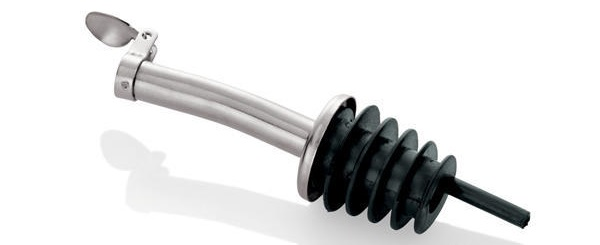
\includegraphics[scale=0.6]{obrazky/nalevac.jpg}
        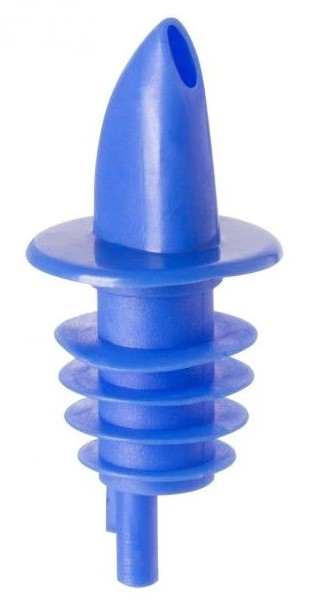
\includegraphics[scale=0.15]{obrazky/nelévač_plast.jpg}
    \end{center}
    \label{nalevačos}
    \caption{Nalévače na alkohol \cite{nalevatko}}
\end{figure}
%modré lavévátko: https://www.alkohol-shop.cz/nalevatko-plastove-modre/

\subsection{Chyba z plnění lahve}
\label{Chyby hustoty}
Pro výpočet objemu (rovnice č. \ref{objem_kapalina}) je nutná znalost hustoty destilátu, pro kterou platí předpis rovnice č. \ref{hustota_kapalina}, kde $m_{max}$ se získá navážením plné neotevřené lahve, $m_{min}$ navážením té stejné prázdné lahve, čímž se eliminuje chyba z rozptylu lahví viz kap. č. \ref{Chyba hmotnosti lahve} (chyby se navzájem odečtou) a $V_{max}$ se stanoví z etikety destilátu, který by měl odpovídat rozdílu $m_{max}$ a $m_{min}$. V této fázi vstupuje do výpočtu chyba plnění, tj. odchylka skutečného objemu od hodnoty uvedené na etiketě.

Podle nařízení EU č. 1169/2011 je v obchodních řetězcích přípustná relativní chyba objemu 1,5 \% pro kapalné produkty o objemu 500–1000 ml, což pro 1000 ml představuje toleranci $\pm$15 ml. V tomto případě by samotná chyba plnění převýšila chybu odměrných válců třídy B o objemu 1 l. Pro ověření byla provedena vlastní měření na 15 lahvích destilátu Amundsen vodka 0,5 l, kde chyba vyšla $\pm$3,65 ml (viz tab. č. \ref{tab:chyba_lahve_a_plnění}). Měřeno váhou s přesností $\pm$0,01 g a přepočteno na objem z hustoty odpovídající měřenému destilátu.


%a přepočteno na objem z hustoty odpovídající směsi vody a ethanolu v poměru 2:1 viz tabulka \ref{tab:chyba_lahve_a_plnění}. Do výpočtu samotné hustoty nám vstupuje chyba  objemu +-3,65 a chyba váhy s kterou jsou měřeny $m_{max}$ a $m_{min}$.

%---------------------------------------------------------------

%Do budoucna je v plánu databázi přesunout na server, kdesi uživatel váhy pouze stahne aktualizovanou databázi, kde je evidovaná hustota destilátu s maximální přesností pro minimalizaci chyby, ale chci dát též uživateli možnost si uložit destilát do databáze za předpokladu, že by měl exotický kousek který by nebyl uloženy v databazi na serveru a to za cenu snížení přesnosti měření tohoto destilátu. 

%Do budoucna je v plánu databázi přesunout na server, aby uživatel nemusel vést databízi a ukládat do ní nové destiláty, možnost toho ale zustane pro případ uložení destilátu, který nebude dostupný v rámci online databáze, tam budou hustoty destilátů měřeny s vyšší přesností(jednorázová investice), důvodem je jednorázová investice, která se finančně nijak nedotýka spotřebitele a navíc hlavním zdrojem chyby systému je právě ze stanovená hustoty, pro minimalizaci chyby. Přesnost váhy zůstane stejná z důvodu pořizovacích nákladů (není důvod si připlácet o několik tisíc korun za možnost naměřit objem o "3 kapky" lépe / není důvod si připlácet o několik tisíc korun za možnost naměřit objem s přesností na 0,01 ml). V případě zanedbání chyby hustoty by celková chyba systému vyšla 

%----------------------------------------------------------------


%Cílem práce je mít databázi uloženou na serveru, kde si uživatel váhy pouze stahne aktualizovanou databázi, kde je evidovaná hustota destilátu s maximální přesností pro minimalizaci chyby, ale chci dát též uživateli možnost si uložit destilát do databáze za předpokladu, že by měl exotický kousek který by nebyl uloženy v databazi na serveru a to za cenu snížení přesnosti měření tohoto destilátu. 

%Poslední možností je, pokud uživatel trvá na vysoké přesnosti a destilát neni uložen v databázi je možné si pořídit vlastní přesné zařízení pro stanovení hustoty kapaliny jako je pyknometr nebo přesná váha + přesný odměrný válec.

%Cílem zařízení je i cenově dostupná možnost pro řešení inventarizace, proto do online databáze budou ukládaná s přesností, která neovlivní výslednou přesnost zařízení. Obsluhu a správu online databáze bude provádět prodejce měřícího systému (já).

\subsection{Chyba váhy}
Posledním klíčovým faktorem je chyba váhy. Jedná se o jedinou chybu, která je ovlivnitelná, proto je nutné na základě již zmíněných chyb výše zvolit přesnost váhy takovou, aby celková přesnost systému nepřesáhla stanovenou hranici $\pm$ 10 ml.


%Teoreticky by nám stačila přesnost vyšší jak +-10g (+-10 ml vody), ale je nutné vzít v potaz i ostaní chyby, které ve výsledku mohou překročit celkovou chybu +-10 ml. Tedy přesnost váhy musí být určena z ohledem na to aby měřící systém jako celek nepřekročil celkovou chybu +-10ml.

Hmotnost se nám ve vzorcích č. \ref{objem_kapalina} a č.  \ref{hustota_kapalina} vyskytuje na 4 místech: \textit{m}, $m_{max}$ a 2x $m_{min}$. Z praktického hlediska bude měření těchto veličin prováděno stejnou váhou. Pro vypočtení přesnosti váhy je nutné znát jak se se jednotlivé chyby v systému šíří a působí na sebe, což je ukázáno na schématu obr. č. \ref{chyby} - jednotlivé proměnné jsou popsané v tab. č. \ref{tab:popis-symbolu}. (V tabulce č.x je vidět výsledná chyba systému v závislosti na různě přesných váhah běžně dostupných na trhu.) V tabulce č. \ref{tab:přesnosti vah} je vidět jak jednotlivé přesnosti běžně dostupných vah na trhu ovlivňují celkovou chybu systému. Hlavním složením destilátů je voda a ethanol, které jsou v různém poměru na základě druhu destilátu. Ethanol má menší hustotu, tedy na jednotku hmotnosti má větší objem než voda, proto byly výpočty stanoveny i pro destilát s obsahem čistého ethanolu. Výsledná přesnost systému se nachází někde mezi chybou stanovenou ethanolem a vodou. Z tabulky č. \ref{tab:přesnosti vah} odpovídá stanovenemu požadavku na přesnost do $\pm$ 10 ml, váha s přesností 0,5 g. 

V příkladu č. \ref{vypočet_objemu} je uveden výpočet pro váhu s přesností d = 0,5 g při hustotě vody. Chyba z orosení lahve nebyla ve výpočtu uvažována. V praxi je lahev vážena bezprostředně po vyjmutí z lednice, takže vysrážená voda na stěně je zanedbatelné hmotnosti (viz tab. \ref{tab:measurement_data}), navíc se dá chyba kompenzovat otřením samotné lahve. Pro stanovení přesnosti systému je využito metody maximální kumulované chyby tzv. worst-case, která uvažuje nejvyšší možné hodnoty dílčích chyb a nezohledňuje jejich pravděpodobnostní rozdělení, na rozdíl od analýzy nejistot podle GUM (Guide to the Expression of Uncertainty in Measurement).

%Na příkladu č. \ref{vypočet_objemu} je vidět konkrétní výpočet pro váhu s přesností d = 0,5 g při hustotě vody. Chyba z orosení lahve nebyla ve výpočtu uvažována. V praxi je lahev před vážením otřena a proces probíhá bezprostředně po vyjmutí z chladu, takže vysrážená voda na stěně nemá měřitelný vliv na hmotnost (viz tab. \ref{tab:measurement_data}). Pro stanovení přesnosti je využito metody chyb měření, které počítají s maximální možnou chybou tzv. "worst-case", která narozdíl on nejistot měření nepočítají s pravděpodobností výskytu chyby.

%Pro výpočet bylo využití klasických metod pro práci s chybami tzv. "worst case", kdy nam vyjde absolutní, největší možná chyba, včetně, do výpočtu jsou započítány i hrubé chyby měření, ale tím, že nám jde jen o hrubý odhad přesnosti, aby příliš "neuskočila" od přesností oměrných válců nám stačí. V případě určení přesnější chyby systému by bylo nutné zvolit stanovení chyby pomocí nejistot, které počítají s pravděpodobností výskytu chyby. Výpočet by byl složitější z důvodu nepřímého měření, který by vedl na parciální derivaci pro výpočet citlivostního koefientu a nutnosti započítat korelaci z důvodu systematických chyb způsobené opakovaným měřením stjného zařízením, výsledkem by ale byla realističtější a menší chyba systému.

%Z tabulky jde vidět, že zvyšování přesnosti váhy o 1 řád přinese zlepšení pouze o $\approx$1 ml.

\begin{figure}[H]
    \begin{center}
        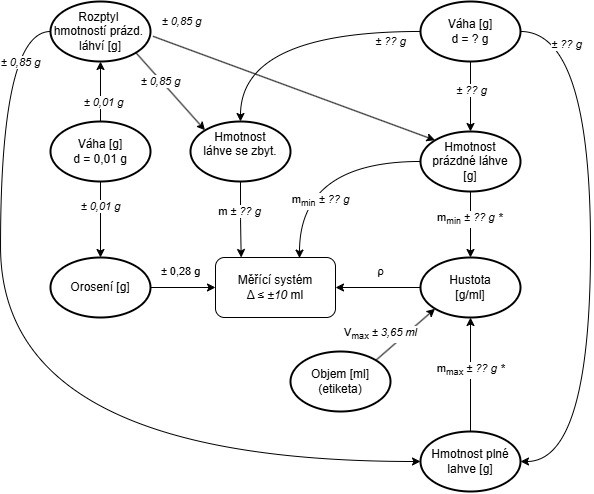
\includegraphics[scale=0.9]{obrazky/Propagace nejistot-Metoda1++.jpg}
    \end{center}
    \caption{Šíření chyb měřicím systémem}
    \label{chyby}
\end{figure}

\begin{table}[H]
    \centering
    \begin{tabular}{|l|l|}
        \hline
        \textbf{Symbol} & \textbf{Popis} \\ \hline \hline
        $m_{\text{min}}$ [g] & Hmotnost prázdné lahve \\ \hline
        $m_{\text{max}}$ [g]& Hmotnost plné lahve \\ \hline
        $m$ [g]& Hmotnost láhve se zbytkovým objemem \\ \hline
        $V_{\text{max}}$ [ml] & Max. objem lahve (etiketa) \\ \hline
        $\rho$ [g/ml]& Hustota kapaliny \\ \hline
        $\Delta_{\rho}$ [g/ml] & Chyba hustoty kapaliny \\ \hline
        $\Delta_m$ [g]& Chyba váhy pro stanovení chyby $\Delta_o$ a $\Delta_\ell$ \\ \hline
        $\Delta_o$ [g]& Chyba z orosení lahve (viz kap. č. \ref{orosení}) \\ \hline
        $\Delta$ [g]& Chyba váhy měřícího systému \\ \hline
        $\Delta_{V_{\text{max}}}$ [ml]& Chyba plnění lahve výrobcem (viz kap. č. \ref{Chyby hustoty}) \\ \hline
        $\Delta_\ell$ [g]& Chyba z rozptylu hmotnosti lahví (viz kap. č. \ref{Chyba hmotnosti lahve}) \\ \hline
        $\Delta_V$ [ml]& Chyba měřicího systému \\ \hline
    \end{tabular}
    %\caption{Popis symbolů ze schématu na obr. č.x a příkladu č.x }
    %\caption{Popis symbolů pro obr. č.x a příklad č.x }
    %\caption{Popis šířících se veličin a chyb měřicího systému}
    \caption{Popis šířících se veličin a chyb měřicím systémem}
    \label{tab:popis-symbolu}
\end{table}

\noindent\textbf{Výpočet hustoty destilátu} 
\smallskip
\newline
Hodnoty $m_{max}$, $m_{min}$ a $V_{max}$ jsou zvoleny, aby odpovídaly hustotě vody $\rho = 0,998$ g/ml v případě použití lahve s objemem 1 l. Hodnoty chyb jsou převzaty z výše uvedených kapitol (viz kap. č. \ref{orosení} až č. \ref{Chyby hustoty}). Souhrnný výpis použitých chyb v tomto příkladu je ukázán v tab. č. \ref{tab:chyby_rozloení}.

\begin{equation}
    \rho \;=\;
\frac{\bigl(m_{\max}+\Delta_{\ell}\bigr)\,\pm\Delta
      \;-\;\bigl(m_{\min}+\Delta_{\ell}\bigr)\,\pm\Delta}
     {V_{\max}\,\pm\Delta_V} = \frac{(m_{\max}-m_{\min})\;\pm\;2\Delta}
     {V_{\max}\,\pm\Delta_V}   
     \label{hustotaa}
\end{equation}
\bigskip
$m_{max}$ a $m_{min}$ se stanoví stejnou lahví, čímž se jejich chyby $\Delta_\ell$ navzájem vyruší.

\begin{equation}
\rho \;=\;
\underbrace{
\frac{(m_{\max}-m_{\min})}{V_{\max}}
}_{\text{nominální hodnota}}
\;\pm\;
\underbrace{
\frac{(m_{\max}-m_{\min})}{V_{\max}}
\left(
   \frac{2\,\Delta}{(m_{\max}-m_{\min})} \;+\; \frac{\Delta_{V_{\max}}}{V_{\max}}
\right)
}_{\text{maximální (worst-case) chyba}}
     \label{objem_kapalinaaa}
\end{equation}

\begin{equation}
\rho = \frac{(1198-200)}{1000}
\;\pm\;
\frac{(1198-200)}{1000}
\left(
   \frac{2 \cdot 0,5}{998} \;+\; \frac{3,65}{1000}
\right) = 0,998 \pm 0,00464 \text{ g/ml}
     \label{objem_kapalinaa}
\end{equation}

\noindent\textbf{Výpočet zbytkového objemu destilátu} 
\smallskip
\newline
Hodnota $m$ je rovna $m_{max}$ (zbytkový objem odpovídá plné lahvi) z důvodu získání nejvyšší relativní chyby, tedy i nejvyšší chyby celého měřicího systému.

\begin{equation}
V \;=\;
\frac{m \pm (\Delta + \Delta_\ell) \;-\; m_{\min} \pm (\Delta + \Delta_\ell)}
     {\rho \;\pm\; \Delta_\rho}\, = 
\frac{\,(m-m_{\min}) \;\pm\; 2(\Delta + \Delta_\ell)}
     {\rho \;\pm\; \Delta_\rho}
 \end{equation}

 \begin{equation}
V \;=\;
\underbrace{
\frac{\,(m-m_{\min})}
     {\rho} 
 }_{\text{nominální hodnota}}
 \pm
 \underbrace{
 \frac{(m-m_{\min})}{\rho}
\left(
   \frac{2\,(\Delta+\Delta_\ell)}{(m-m_{\min})} \;+\; \frac{\Delta_\rho}{\rho}
\right)
}_{\text{maximální (worst-case) chyba}}
 \end{equation}

 \begin{equation}
V \;=\;
\frac{(1198-200)}{0,998}
\pm
 \frac{(1198-200)}{0,998}
\left(
   \frac{2\,(0,5+0,85)}{(1198-200)} \;+\; \frac{0,00464}{0,998}
\right) = 1000 \pm 7,35 \text{ ml}
\label{vypočet_objemu}
 \end{equation}

% Requires: \usepackage{amsmath}
\begin{table}[h]
    \centering
    \begin{tabular}{|l|c|c|c|}
        \hline
        \textbf{Chyba} & \textbf{Hodnota} & \textbf{Příspěvek [ml]} & \textbf{Rel. Příspěvek [\%]} \\
        \hline \hline
        $\Delta V_{\text{max}}$ & $\pm 3{,}65 \, \text{ml}$ & 3{,}65 & 49,7 \\
        \hline
        $\Delta$ & $\pm 0{,}5 \, \text{g}$ & $4\Delta / \rho_{\text{voda}} = 2$ & 27,2 \\
        \hline
        $\Delta_\ell$ & $\pm 0{,}85 \, \text{g}$ & $2\Delta_\ell / \rho_{\text{voda}} = 1{,}7$ & 23,1 \\
        \hline
        $\Delta_V$ & $\pm 7{,}35 \, \text{g}$ & 7,35 & 100 \\
        \hline
    \end{tabular}
    \caption{Rozložení "worst-case“ chyb v systému – absolutní a relativní podíl}
    %\caption{Přehled chybových příspěvků a jejich relativní přispění}
    \label{tab:chyby_rozloení}
\end{table}

\begin{table}[H]
    \centering
    \begin{tabular}{|c|c|c|}
        \hline
        \begin{tabular}[c]{@{}c@{}}Přesnost \\ váhy [$\pm$ g]\end{tabular} & \begin{tabular}[c]{@{}c@{}}Přesnost systému \\ (voda) [$\pm$ ml]\end{tabular} & \begin{tabular}[c]{@{}c@{}}Přesnost systému \\ (ethanol) [$\pm$ ml]\end{tabular}\\ \hline \hline
         1 & 9,35 - 11,4 & 11.9 - 12,66\\ \hline
         0,5 & 7.35 - 9,90 & 9.32 - 10,76\\ \hline
         0,1 & 5.75 - 8,70 & 7.29 - 9,24\\ \hline
         0,01 & 5.39 - 8,43 & 6.83 - 8,89\\ \hline
    \end{tabular}
    \caption{Přesnost měřicího systému v závislosti na přesnosti váhy a měřeném médiu}
    \label{tab:přesnosti vah}
\end{table}


%za Δ dosadíme přesnosti běžně dostupných vah.
Největší podíl na celkové chybě systému má chyba $\Delta_{V_{\text{max}}}$ viz tab. č. \ref{tab:chyby_rozloení}. V případě výpočtu objemu za pomocí dat z online databáze, kde je hustota vedena přesně, by její chyba odpadla. Chyba systému by pak odpovídala předpisu č. \ref{chyba_objemu} - Opětovné vynechání chyby z orosení láhve. Navíc pokud dosadíme znovu váhu s přesností 0,5 g, tak nám nyní vyjde přesnost značně vyšší a to $\pm$1,35 ml pro vodu (viz příklad č. \ref{chyba_objemu_vyčislení}).

\begin{equation}
\Delta_V = \frac{\Delta + \Delta_\ell}{\rho_{voda}}
\label{chyba_objemu}
\end{equation}

 \begin{equation}
\Delta_V = \frac{0,5 + 0,85}{0,998} = 1,35 \text{ ml}
\label{chyba_objemu_vyčislení}
\end{equation}
----------------------------------------------------------------------------------------------------

xxxxxxxxxxxxxxxxxxxxxxxxxxxxxxxxxxxxxxxxxxxxxxxxxxxxxxxxxxxxxxxxxxxxxx

------------------------------------------------------------------------------------------------


%\begin{equation}
%    \pm m = \pm 5 \cdot 0.789 \, \left[\mathrm{g}\right] \label{objem_kapalina}
%\end{equation}



%\subsection{Stanovení přesnosti váhy na základě }
%Propagace nejistot pro měřící metodu A
%\subsection{Výpočet hustoty přes hmotnost lahve a stanovení přesnosti váhy}

%Zde dominantní chybu tvoří objem kapaliny, i když nám z měření vyšla chyba pouze +-xx ml, tak budem počítat z maximálně možnou dle normy ISOXXX.

%Výslednou chybu dokáže ovlivnit zda m\_min a m\_max budem měřit ze stejné láhve či nkoli. v případě stejné láhve se nám vykompenzuje chyba způsobená rozptylem hmotností lahví (+- 0,85g)

%I když chyba systému je zanedbatelná pro inevnturní účely v praxi bude systém připojen k online databázi, aby uživatel nemusel vést databízi a ukládat do ní nové destiláty, možnost toho ale zustane pro případ uložení destilátu, který nebude dostupný v rámci online databáze, tam budou hustoty destilátů měřeny s maximální přesností(jednorázová investice), důvodem je jednorázová investice, která se finančně nijak nedotýka spotřebitele a navíc hlavním zdrojem chyby systému je právě ze stanovená hustoty, pro minimalizaci chyby. Přesnost váhy zůstane stejná z důvodu pořizovacích nákladů (není důvod si připlácet o několik tisíc korun za možnost naměřit objem o "3 kapky" lépe / není důvod si připlácet o několik tisíc korun za možnost naměřit objem s přesností na 0,01 ml). V případě zanedbání chyby hustoty by celková chyba systému vyšla 



%\begin{figure}[H]
%    \begin{center}
%        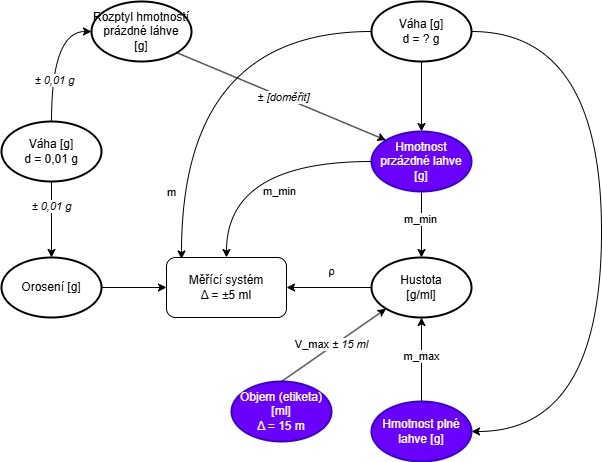
\includegraphics[scale=0.6]{obrazky/Propagace nejistot-Metoda1+.jpg}
%    \end{center}
%    \caption{Propagace nejistot - Výpočet hustoty pomocí plné láhve}
%\end{figure}
%
%//Tabulka ze vstupními parametry a jejich podílem chyby
%// nebo proste jen udělat tabulku a chyb a jejich podíl chyby


%řesnosti váhy}
%
%řednictím odměrného válce, který bude dostačující přesnosti, aby celý systém splňoval kritérium přesnosti. Přesnost válce a váhy by vůči sobě neměly být příliš rozdílný, aby měli na chybu stejný vliv (ovlivnily chybu ve stejném řádu - tedy se nejlépe navzájem vyrovnají). (pokud válec bude větší přesnosti a váha menší, přesnost válce bude automaticky kompenzována na přesnost váhy a naopak.). Dostupné válce na trhu se řídí zmíněnou normou ISOxxx. Podmínkou výběru válce je absolutní chyba pod +-5ml, tedy válce s menším objeme. Z dostupných válcu na trhu je nejvhodnějším kadinátem 250 ml válec s přesností +-1ml, kde jeho relativní chyba činí 0,4\% tedy jedná se o nejpřesnější válec na velikost vlastního objemu. Tedy pokud budem stanovovat hustotu ze vzorku pokrývající max objem válce a váhou stejné přesnosti výjde nám nejmenší relativní chyba hustoty.
%
%hustší kapa-
%kapalina bude
%vážit méně na jednotku objemu, v našem případě 10 ml. Tudíž nás zajímá, která
%složka destilátu má nejmenší hustotu. Ve své podstatě bude měřen pouze ethanol
%a voda, co se týče příměsí pro dochucení, tak ty jsou větší hustoty, proto přesnost váhy vztáhneme k ethanolu, i když nikdy nebudeme měřit 100\% ethanol, ale jeho směs s vodou a dalšími příměsi.

%Nakonec byl vytvořen Python script, který kombinuje dotupné přesnosti odměrných válců a vah. Z důvodu, jak bylo zmíněné už u válce nezáleží na absolutní chybě ale relativní, tudíž je možné využít celé spektrum dostupných válců, které se relativně jen mírně liší, díky skriptu ne že jsem schopen najít nejpřesnější kombinaci, ale vidím všechy ostatní kombinace pro přehled a jak působí na měřící systém.

%\begin{equation}
%    \pm m = \pm 5 \cdot 0.789 \, \left[\mathrm{g}\right] \label{objem_kapalina}
%\end{equation}

\begin{table}[h]
\centering
\caption{Rozpočet „worst-case“ chyb – absolutní i relativní podíl}
\renewcommand{\arraystretch}{1.15}
\begin{tabular}{@{}lcccc@{}}
\toprule
\textbf{Zdroj} & \textbf{Hodnota} & \textbf{Koef.} & \textbf{Příspěvek [ml]} & \textbf{Rel. podíl [\%]}\\
\midrule
Chyba plnění při~kalib.        & $\pm3{,}35\ \mathrm{ml}$ & $2$ & $6{,}70$ & $67{,}7$\\
Chyba váhy (\(\Delta\))        & $\pm0{,}50\ \mathrm{g}$ & $3S$ & $1{,}50$ & $15{,}2$\\
Rozptyl prázdných lahví (\(\Delta_\ell\))
                               & $\pm0{,}85\ \mathrm{g}$ & $2S$ & $1{,}70$ & $17{,}1$\\
\midrule
\multicolumn{3}{r}{\textbf{Celkem}} &
\(\boxed{\Delta V_{\text{max}} = 9{,}90\ \mathrm{ml}}\) & $100$\\
\bottomrule
\end{tabular}
\label{tab:worst_case_budget_rel}
\end{table}


\begin{table}[h]
\centering
\caption{Dosazené hodnoty a jejich příspěvek do maximální chyby objemu}
\renewcommand{\arraystretch}{1.2}
\begin{tabular}{@{}lccccc@{}}
\toprule
\textbf{Symbol} & \textbf{Popis} & \textbf{Hodnota} & \textbf{Příspěvek}\\
\midrule
$V_{\max}$      & jmenovitý objem lahve           & $1000\ \text{ml}$  & – \\
$m_{\max}$      & hmotnost plné lahve (kalibr.)   & $1180\ \text{g}$   & – \\
$m_{\min}$      & hmotnost prázdné lahve (kalibr.)& $180\ \text{g}$    & – \\
$S=\dfrac{V_{\max}}{m_{\max}-m_{\min}}$
                & převod $\,\bigl[\text{g}\rightarrow\text{ml}\bigr]$
                                                   & $1,000\ \text{ml·g}^{-1}$ & – \\[4pt]
\(\Delta V_{\text{plnění}}\)
                & chyba plnění při kalibraci      & $\pm3,35\ \text{ml}$ &
\(2\,\Delta V_{\text{plnění}} = 6,70\ \text{ml}\) \\

\(\Delta\)      & chyba váhy (každé vážení)       & $\pm0,50\ \text{g}$ &
\(3\,\Delta\,S = 1,50\ \text{ml}\) \\

\(\Delta_{\ell}\)
                & rozptyl hmotností lahví         & $\pm0,85\ \text{g}$ &
\(2\,\Delta_{\ell}\,S = 1,70\ \text{ml}\) \\
\midrule
\multicolumn{3}{r}{\textbf{Celková maximální chyba}} &
\(\boxed{\Delta V_{\text{max}} = 9,90\ \text{ml}}\) \\
\bottomrule
\end{tabular}
\label{tab:worst_case_budget}
\end{table}


\[
\Delta\rho_{\max}= \rho_{\mathrm{DB}}
\left(
   \frac{2\Delta}{m_{\max}-m_{\min}}
  +\frac{\Delta V_{\max}}{V_{\max}}
\right)
\]

\[
\Delta V_{\max}= 2\,\Delta V_{\max}^{\text{plnění}}
               +\frac{3\Delta\,V_{\max}}{m_{\max}-m_{\min}}
\tag{A}
\]


\[
\Delta V_{\max}
  = 2\,\Delta V_{\max}^{\text{plnění}}
  + \frac{(3\Delta + 2\Delta_{\ell})\,V_{\max}}
         {m_{\max}-m_{\min}}
\tag{B}
\]


\begin{equation}
    \rho \;=\;
\frac{\bigl(m_{\max}+\Delta_{\ell}\bigr)\,\pm\Delta
      \;-\;\bigl(m_{\min}+\Delta_{\ell}\bigr)\,\pm\Delta}
     {V_{\max}\,\pm\Delta_V} = \frac{(m_{\max}-m_{\min})\;\pm\;2\Delta}
     {V_{\max}\,\pm\Delta_V}   
     \label{hustotdda}
\end{equation}



\begin{equation}
\rho \;=\;
\underbrace{
\frac{(m_{\max}-m_{\min})}{V_{\max}}
}_{\text{nominální hodnota}}
\;\pm\;
\underbrace{
\frac{(m_{\max}-m_{\min})}{V_{\max}}
\left(
   \frac{2\,\Delta}{(m_{\max}-m_{\min})} \;+\; \frac{\Delta_{V_{\max}}}{V_{\max}}
\right)
}_{\text{maximální (worst-case) chyba}}
     \label{objem_kapasdalina}
\end{equation}

\begin{equation}
\rho = \frac{998}{1000}
\;\pm\;
\frac{998}{1000}
\left(
   \frac{2 \cdot 0,5}{998} \;+\; \frac{3,65}{1000}
\right) = 0,998 \pm 0,00464 ml/g
     \label{objem_kapasdalina}
\end{equation}

\begin{equation}
V \;=\;
\frac{m \pm (\Delta + \Delta_\ell) \;-\; m_{\min} \pm (\Delta + \Delta_\ell)}
     {\rho \;\pm\; \Delta_\rho}\, = 
\frac{\,(m-m_{\min}) \;\pm\; 2(\Delta + \Delta_\ell)}
     {\rho \;\pm\; \Delta_\rho}
 \end{equation}

 \begin{equation}
V \;=\;
\underbrace{
\frac{\,(m-m_{\min})}
     {\rho} 
 }_{\text{nominální hodnota}}
 \pm
 \underbrace{
 \frac{(m-m_{\min})}{\rho}
\left(
   \frac{2\,(\Delta+\Delta_\ell)}{(m-m_{\min})} \;+\; \frac{\Delta_\rho}{\rho}
\right)
}_{\text{maximální (worst-case) chyba}}
 \end{equation}

 \begin{equation}
V \;=\;
\frac{(1198-200)}{0,998}
\pm
 \frac{(1198-200)}{0,998}
\left(
   \frac{2\,(0,5+0,85)}{(1198-200)} \;+\; \frac{0,00464}{0,998}
\right) = 1000 \pm 7,35 ml
 \end{equation}



%\begin{table}[h]
%\centering
%  \begin{tabular}{c c c c}
%    \toprule
%    \textbf{Popis} &
%    \textbf{Symbol} &
%    \textbf{Hodnota} &
%    \textbf{Příspěvek {[}ml{]}} &
%    \textbf{rel. příspěvek {[}\%{]}} \\ \midrule
%    Hmotnost prázdné láhve              & $m_{\min}$ & $180\;\text{g}$          & --      & --   \\
%    Hmotnost plné láhve                 & $m_{\max}$ & $1180\;\text{g}$         & --      & --   \\
%    Hmotnost láhve se zbytkovým objemem & $m$        & $m = m_{\max}$           & --      & --   \\
%    Max. objem láhve (etiketa)          & $V_{\max}$ & $1000\;\text{ml}$        & --      & --   \\
%    Hustota kapaliny (voda)             & $\rho$     & $1000\;\text{g\,ml}^{-1}$& --      & --   \\
%    Chyba hustoty kapaliny              & $\Delta\rho$ & --                     & --      & --   \\[2pt]
%    Chyba váhy pro stanovení $\Delta_o,\,\Delta_\ell$ & $\Delta_m$ & $\pm 0{,}01\;\text{g}$ & -- & -- \\[2pt]
%    Chyba z orosení láhve (včetně $\Delta_m$) & $\Delta_o$ & $\pm 0{,}28\;\text{g}$ & -- & -- \\[4pt]
%    Chyba váhy měřicího systému         & $\Delta$   & $\pm 3{,}35\;\text{ml}$  & $(4\Delta)/\rho = 2,00$ & 27,2 \\
%    Chyba plnění láhve výrobcem         & $\Delta V_{\max}$ & $\pm 3{,}65\;\text{ml}$ & $\Delta_m = 3,65$ & 49,7 \\
%    Chyba z rozptylu hmotnosti láhví \newline (včetně $\Delta_m$) & $\Delta_\ell$ & $\pm 0{,}85\;\text{g}$ & $2\Delta_\ell/\rho = 1,70$ & 23,1 \\[4pt]
%    \textbf{Chyba měřicího systému}     & $\Delta V$ & -- & \textbf{7,35} & \textbf{100} \\ \bottomrule
%  \end{tabular}
%  \caption{Rekapitulace složek worst-case chyby měřicího systému.}
%\end{table}

% Requires: \usepackage{array}

%\begin{table}[h]
%    \centering
%    \begin{tabular}{|>{\raggedright}p{4cm}|c|c|c|c|}
%    \hline
%    \textbf{Popis} & \textbf{Symbol} & \textbf{Hodnota} & \textbf{Příspěvek [ml]} & \textbf{rel. Příspěvek [\%]} \\ \hline
%    Hmotnost prázdné láhve & $m_\text{min}$ & 180 g & - & - \\ \hline
%    Hmotnost plné láhve & $m_\text{max}$ & 1180 g & - & - \\ \hline
%    Hmotnost láhve se zbytk. Objemem & $m = m_\text{max}$ & - & - & - \\ \hline
%    Max. objem láhve (etiketa) & $V_\text{max}$ & 1000 ml & - & - \\ \hline
%    Hustota kapaliny (voda) & $\rho$ & 1000 g/ml & - & - \\ \hline
%    \textbf{Chyba hustoty kapaliny} & $\Delta_{\rho}$ & & & \\ \hline
%    Chyba váhy pro stanovení $\Delta_m$ a $\Delta_{\rho}$ & $\Delta_m$ & $\pm0,01$ g & & \\ \hline
%    Chyba z orosení láhve (viz kap. č.) & & & & \\ \hline
%    včetně chyby váhy $\Delta_m$ & $\pm$ & $3,35$ ml & & \\ \hline
%    Chyba váhy měřicího systému & $\Delta$ & & & \\ \hline
%    včetně chyby váhy $\Delta_m$ & $\pm 0,28$ g & $\frac{44}{\rho^2} =$ & $27,2$ \\ \hline
%    Chyba plnění láhve výrobcem (viz kap. č. x) & $\Delta V_\text{max}$ & $\pm3,65$ ml & & \\ \hline
%    včetně chyby váhy $\Delta_m$ & & & $49,7$ \\ \hline
%    Chyba z rozptylu hmotnosti láhví (viz kap. č. x) & & & & \\ \hline
%    včetně chyby váhy $\Delta_m$ & $\pm0,85$ g & $\pm1,97$ & $23,1$ \\ \hline
%    \textbf{Chyba měřicího systému} & $\Delta V$ & & $7,35$ & $100$ \\ \hline
%    \end{tabular}
%    \caption{Tabulka chyb a příspěvků měření}
%    \label{tab:chyby-prispevky}
%\end{table}

%%%%%%%%%%%%%%%%%%%%%%%%%%%%%%%%%%%%%%%%%%%%%%%%%%%

%\[
%\rho \;=\;
%\frac{\bigl(m_{\max}+\Delta_{\ell}\bigr)\,\pm\Delta
%      \;-\;\bigl(m_{\min}+\Delta_{\ell}\bigr)\,\pm\Delta}
%     {V_{\max}\,\pm\Delta_V} = \frac{(m_{\max}-m_{\min})\;\pm\;2\Delta}
%     {V_{\max}\,\pm\Delta_V}   
%\]
%
%\(m_{min}\) ...hmotnost prázdné láhve \([\mathrm{g}]\)
%
%\(m_{max}\) ...hmotnost plné láhve \([\mathrm{g}]\)
%
%\(\rho\) ...hustota kapaliny \([\mathrm{g/ml}]\)
%
%\(\Delta\) ...chyba váhy \([\mathrm{g}]\)
%
%\(\Delta_\ell\) ...chyba z rozptylu hmotnosti prázdných láhví \([\mathrm{g}]\)
%
%\(\Delta_V\) ...chyba objemu plné láhve (etiketa) \([\mathrm{g}]\)
%
%\[
%m_{\rho} \;=\; m_{\max} \;-\; m_{\min}
%\]
%
%\(m_{\rho}\) ...hmotnost kapaliny pro stanovení hustoty\([\mathrm{g}]\)
%
%\[
%\rho \;=\;
%\frac{m_{\rho} \,\pm\, 2\Delta}
%     {V_{\max} \,\pm\, \Delta_{V_{\max}}} = \frac{m_{\rho}}{V_{\max}}
%\;\pm\;
%\frac{m_{\rho}}{V_{\max}}
%\left(
%   \frac{2\,\Delta}{m_{\rho}} \;+\; \frac{\Delta_{V_{\max}}}{V_{\max}}
%\right)
%\]


%\[
%V \;=\;
%\frac{%
%      m \,\pm\, (\Delta + \Delta_\ell)
%      \;-\;
%      m_{\min} \,\pm\, (\Delta + \Delta_\ell)
%     }{%
%      \rho \,\pm\, \Delta_\rho
%     }.
%\]
%
%V ...objem kapaliny
%
%m ...hmotnost láhve se zbytkovou kapalinou \([\mathrm{kg}]\)
%
%\(\Delta_\rho\) ...chyba hustoty \([\mathrm{g/ml}]\)
%
%\[
%m_{\mathrm{zb}} \;=\; m \;-\; m_{\min}\,.
%\]
%
%\(m_{zb}\) ...hmotnost zbytkové kapaliny v láhvi \([\mathrm{g}]\)
%
%\[
%V \;=\;
%\frac{\,m_{\mathrm{zb}} \;\pm\; 2(\Delta + \Delta_\ell)}
%     {\rho \;\pm\; \Delta_\rho}\,.
%\]
%
%\begin{center}    
%\boxed{%
%V \;=\;
%\frac{%
%      \bigl[m - m_{\min}\bigr]
%      \,\pm\, 2\bigl(\Delta + \Delta_{\ell}\bigr)}%
%     {%
%      \dfrac{m_{\max}-m_{\min}}{V_{\max}}
%      \,\pm\,
%      \dfrac{m_{\max}-m_{\min}}{V_{\max}}
%      \!\left(
%        \dfrac{2\Delta}{m_{\max}-m_{\min}}
%        +\dfrac{\Delta_{V_{\max}}}{V_{\max}}
%      \right)}%
%}\tag{V\text{-full}}
%\end{center}
%
%\begin{center}  
%\boxed{
%V \;=\;
%\frac{%
%      V_{\max}
%      \bigl[m - m_{\min} \,\pm\, 2(\Delta + \Delta_{\ell})\bigr]}%
%     {%
%      (m_{\max}-m_{\min})
%      \left[
%        1
%        \,\pm\,
%        \left(
%          \dfrac{2\Delta}{m_{\max}-m_{\min}}
%          +\dfrac{\Delta_{V_{\max}}}{V_{\max}}
%        \right)
%      \right]}%
%\tag{V\text{-simp}}}
%\end{center}  
%
%\boxed{
%V
%=
%\underbrace{\frac{m-m_{\min}}{m_{\max}-m_{\min}}\,V_{\max}}_{\text{nominalní hodnota}}
%\;\pm\;
%\underbrace{\Bigl[
%      2\,\Delta_{V_{\text{max}}}
%      \;+\;
%      \bigl(3\,\Delta+2\,\Delta_{\ell}\bigr)\,
%      \frac{V_{\max}}{m_{\max}-m_{\min}}
%\Bigr]}_{\text{maximální (worst-case) chyba}}
%
%\tag{V\text{-simp}}}
%
%\bigskip
%Ukázka výpočtu chyby měřicího systému pro $\Delta$ = 0,5 g, $\rho$ = hustota vody = 1 g/ml (V$_{max}$ = 1 l, m\_max = 1200 g a m\_min = 200 g), $\Delta_\ell$ = 0,85 [\ref{Chyba hmotnosti lahve}], $\Delta_{V_{\text{max}}}$ = 3,65 ml [\ref{Chyby hustoty}]
%
%\[
%\Delta_V = 2\,\Delta_{V_{\text{max}}}
%      \;+\;
%      \bigl(3\,\Delta+2\,\Delta_{\ell}\bigr)\,
%      \frac{V_{\max}}{m_{\max}-m_{\min}}
%\]
%
%\[
%\Delta_V = 2 \cdot 3,65
%      \;+\;
%      (3\cdot0,5+2\cdot0,85)\,
%      \cdot\underbrace{\frac{1000}{1200-200}}_{\text{= 1 $\simeq \rho_{voda}$}}=\pm 9,90 ml
%\]